
Event are required to pass a preselection described in section \ref{subsec:presel} and summarized in table \ref{tbl:selection}. Those that pass this preselection are divided into various fit regions described in section \ref{subsec:regions}, based on the number of jets in the event, and the b-tag score of those jets.

%--------------------------- 
\subsection{Event Preselection}
\label{subsec:presel}
%--------------------------- 

Events are required to include exactly three reconstructed light leptons passing the requirement described in \ref{subsec:leps}, which have a total charge of $\pm$1. As the opposite sign lepton is found to be prompt the vast majority of the time \cite{ttH_paper}, it is required to be loose and isolated, as defined though the standard \verb|isolationFixedCutLoose| working point supported by combined performance groups. The same sign leptons are required to be very tight, as per the recommended \verb|isolationFixedCutTight|.

The leptons are ordered in the analysis code as 0, 1, and 2. Lepton 0 is the lepton whose charge is opposite the other two. Lepton 1 is the lepton closest to the opposite charge lepton, i.e. the smallest $\Delta R$, leaving lepton 2 as the lepton further from the opposite charge lepton. Lepton 0 is required to have $p_T > 10$ GeV, while the same sign leptons, 1 and 2, are required to have $p_T > 20$ GeV to reduce the contribution of non-prompt leptons.  

The invariant mass of at least one pair of opposite sign, same flavor leptons is required to fall within 10 GeV of the mass of the Z boson, 91.2 GeV. Events where one of the opposite sign pairs have an invariant mass less than 12 GeV are rejected in order to suppress low mass resonances. %Further, events where the trilepton mass falls within 5 GeV of the Z mass are rejected to remove Z events that include conversions.

An additional requirement is placed on the missing transverse energy, $E^{miss}_T$ > 20 GeV, and the transverse mass of the $W$ candidate, $m(E^{miss}_T + l_{other}) > 30$ GeV, where $E^{miss}_T$ is the missing transverse energy, and $l_{other}$ is the lepton not included in the Z-candidate. 

Events are required to have one or two reconstructed jets passing the selection described in section \ref{subsec:jets}. Events with more than two jets are rejected in order to reduce the contribution of backgrounds such as $t\bar{t}Z$ and $t\bar{t}W$, which tend to have higher jet multiplicity. 

\begin{table}[H]
    \centering
    \begin{tabular}{l}
        \hline\hline
        Event Selection\\
        \hline 
        Exactly three leptons with charge $\pm$1 \\
        Two same-charge leptons with $p_T$ $>$ 20 GeV \\
        One opposite charge lepton with $p_T$ $>$ 10 GeV \\
        $m(l^+l^-)$ within 10 GeV of 91.2 GeV \\
        Transverse mass of W-candidate, $m_T(E_T^{miss} + lep_{other})$ $>$ 30 GeV \\
        Missing transverse energy, $E_T^{miss} >$ 20 GeV \\
        One or two jets with $p_T$ $>$ 25 GeV \\
        \hline\hline
    \end{tabular}
    \caption{Summary of the selection applied to events for inclusion in the fit}
    \label{tbl:selection}
\end{table}

The event yields in the preselection region for both data and Monte Carlo are summarized in table \ref{tab:evt_yields}, which shows good agreement between data and Monte Carlo, and demonstrates that this region consists primarily of WZ events. The WZ events are split into WZ + b, WZ + c, and WZ + l based on the truth flavor of the heaviest associated jet in the event. Specifically, this determination is made based on the \verb!HadronConeExclTruthLabelID! of the jet. That is, WZ + l events contain no charm and b jets at truth level, WZ + c contain at least one truth charm and no b-jets, and WZ + b contains at least one truth b-jet. 

\begin{table}[H]
    \centering
        \begin{center}
\begin{tabular}{|c|c|}
\hline
Process & Events \\
\hline 
  $WZ + b$   & 167.6 $\pm$ 6.5 \\
  $WZ + c$   & 1080 $\pm$ 40 \\
  $WZ + l$   & 7220 $\pm$ 310 \\
  Other VV   & 850 $\pm$ 140 \\
  $t\bar{t}W$   & 16.8 $\pm$ 2.3 \\
  $t\bar{t}Z$   & 115 $\pm$ 17 \\
  rare Top   & 2.2 $\pm$ 0.1 \\
  Single top   & 0.10 $\pm$ 0.45 \\
  Three top   & 0.01 $\pm$ 0.01 \\
  Four top   & 0.02 $\pm$ 0.01 \\
  $t\bar{t}WW$   & 0.23 $\pm$ 0.05 \\
  $Z+\text{jets}$   & 600 $\pm$ 260 \\
  $V+\gamma$   & 37 $\pm$ 54 \\
  $tZ$   & 190 $\pm$ 70 \\
  $tW$   & 5.5 $\pm$ 1.2 \\
  $WtZ$   & 25.8 $\pm$ 1.1 \\
  $VVV$   & 26.2 $\pm$ 0.9 \\
  $VH$   & 94 $\pm$ 7 \\
  $t\bar{t}$   & 108.68 $\pm$ 8 \\
  $t\bar{t}H$   & 4.3 $\pm$ 0.5 \\
\hline
  Total  & 10600 $\pm$ 530 \\
\hline
  Data   & 10574 \\
\hline 
\end{tabular} 
\caption{Event yields in the preselection region at 139.0 $fb^{-1}$} 
\end{center} 


    %\caption{Data and MC yields after the event selection requiring three leptons, one or two jets, $E^{miss}_T$ > 20 GeV, and $m(E^{miss}_T + l_{other}) > 30$ GeV selection has been applied.}
    \label{tab:evt_yields}
\end{table}

Here Other $VV$ represents diboson processes other than WZ, and consists predominantly of $ZZ\rightarrow llll$ events where one of the leptons is not reconstructed.

Simulations are further validated by comparing the kinematic distributions of the Monte Carlo with data, which are shown in figures \ref{kin:inclusive}. Here, bins with 5\% or more WZ+b are blinded.

%textbf{There is some discrepancies between data and MC, particularly in the low MET and low lepton $p_T$ regions, which are being investigated. This is suspected to be the result of underestimating the fake contribution, possibly because of several missing Z+jets simulation files.}

\begin{figure}[H]
    \centering
    \textbf{WZ Fit Region - Inclusive}\\
    \subfigure[]{\includegraphics[width=.29\linewidth]{regions/plots_inclusive/Plots/lead_jetPt.png}}%
    \subfigure[]{\includegraphics[width=.29\linewidth]{regions/plots_inclusive/Plots/lep_Pt_0.png}}%
    \subfigure[]{\includegraphics[width=.29\linewidth]{regions/plots_inclusive/Plots/lep_Pt_1.png}}\\      
    \subfigure[]{\includegraphics[width=.29\linewidth]{regions/plots_inclusive/Plots/lep_Pt_2.png}}%
    \subfigure[]{\includegraphics[width=.29\linewidth]{regions/plots_inclusive/Plots/MET.png}}%
    \subfigure[]{\includegraphics[width=.29\linewidth]{regions/plots_inclusive/Plots/Mll01.png}}\\
    \subfigure[]{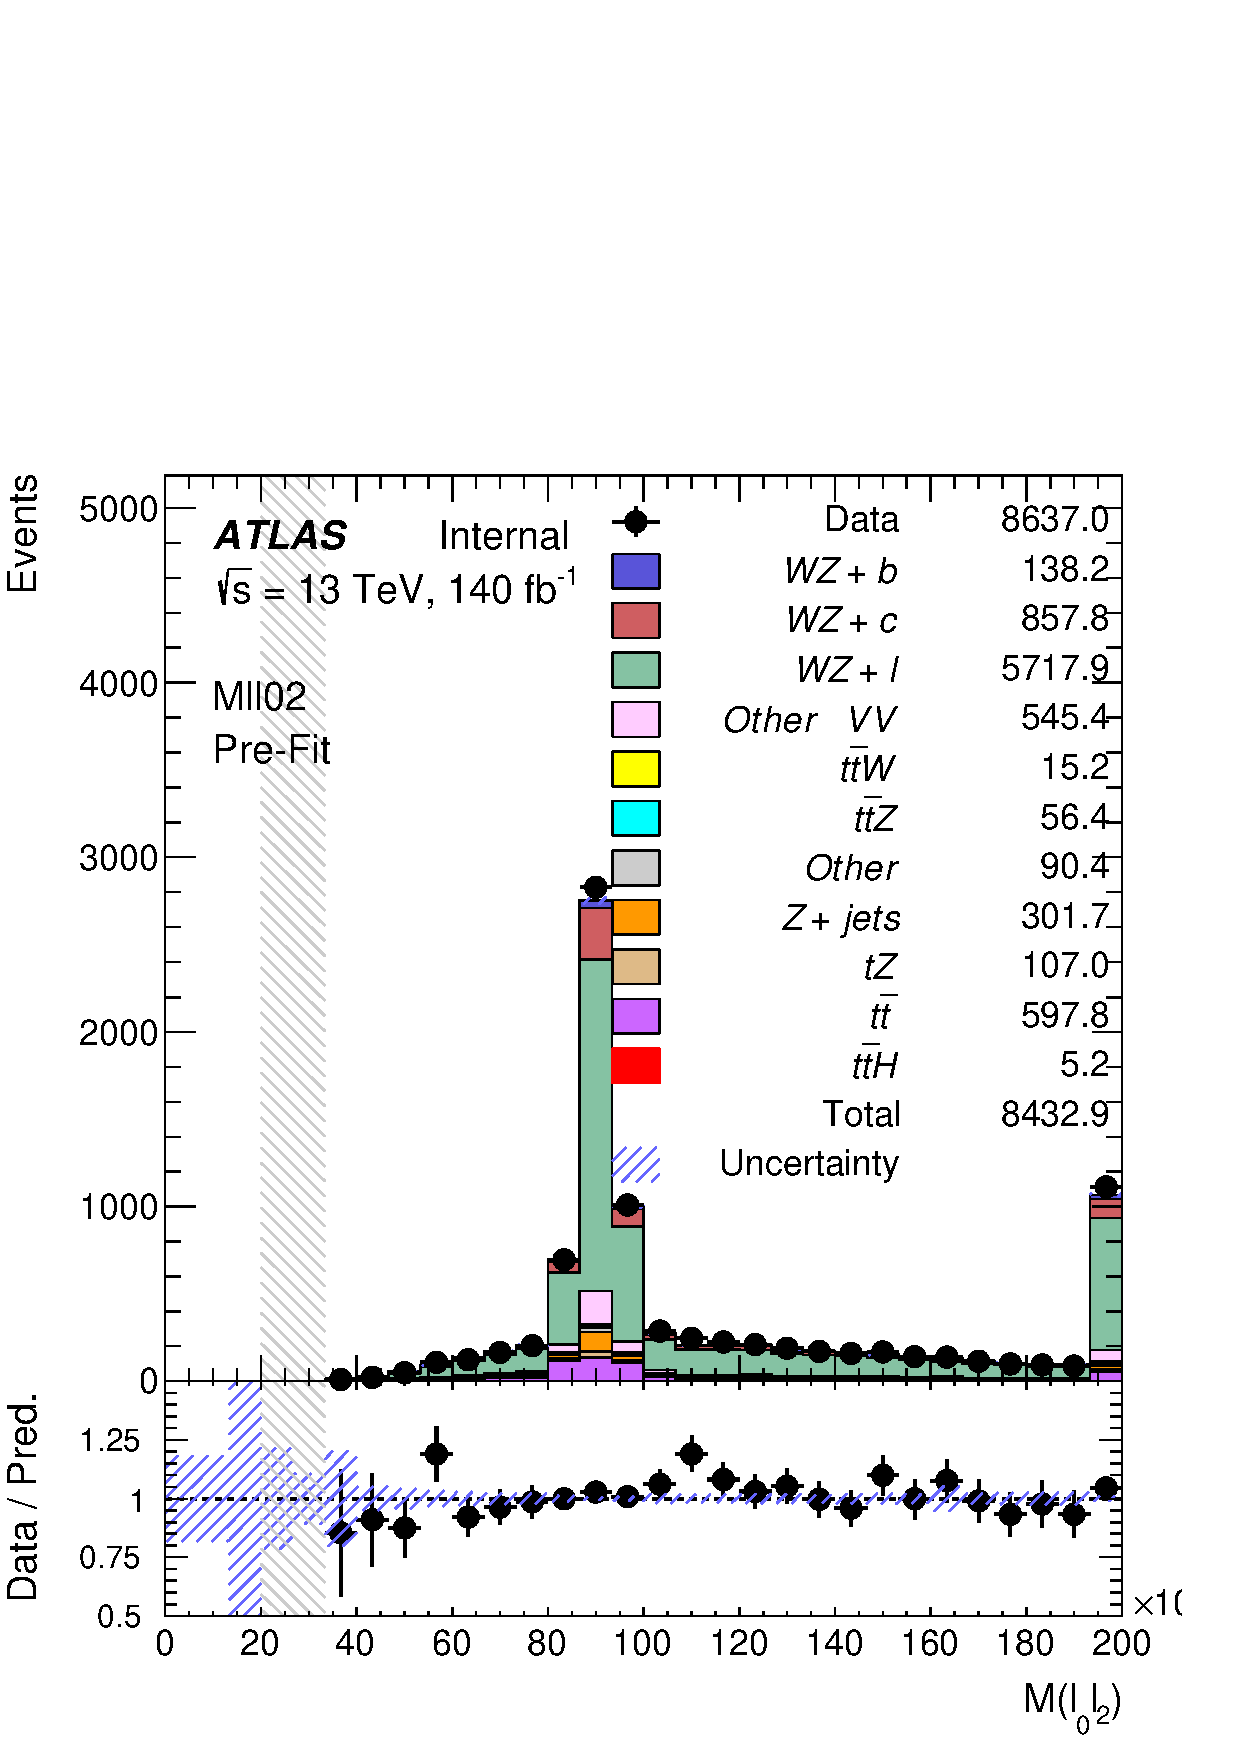
\includegraphics[width=.29\linewidth]{regions/plots_inclusive/Plots/Mll02.png}}%
    \subfigure[]{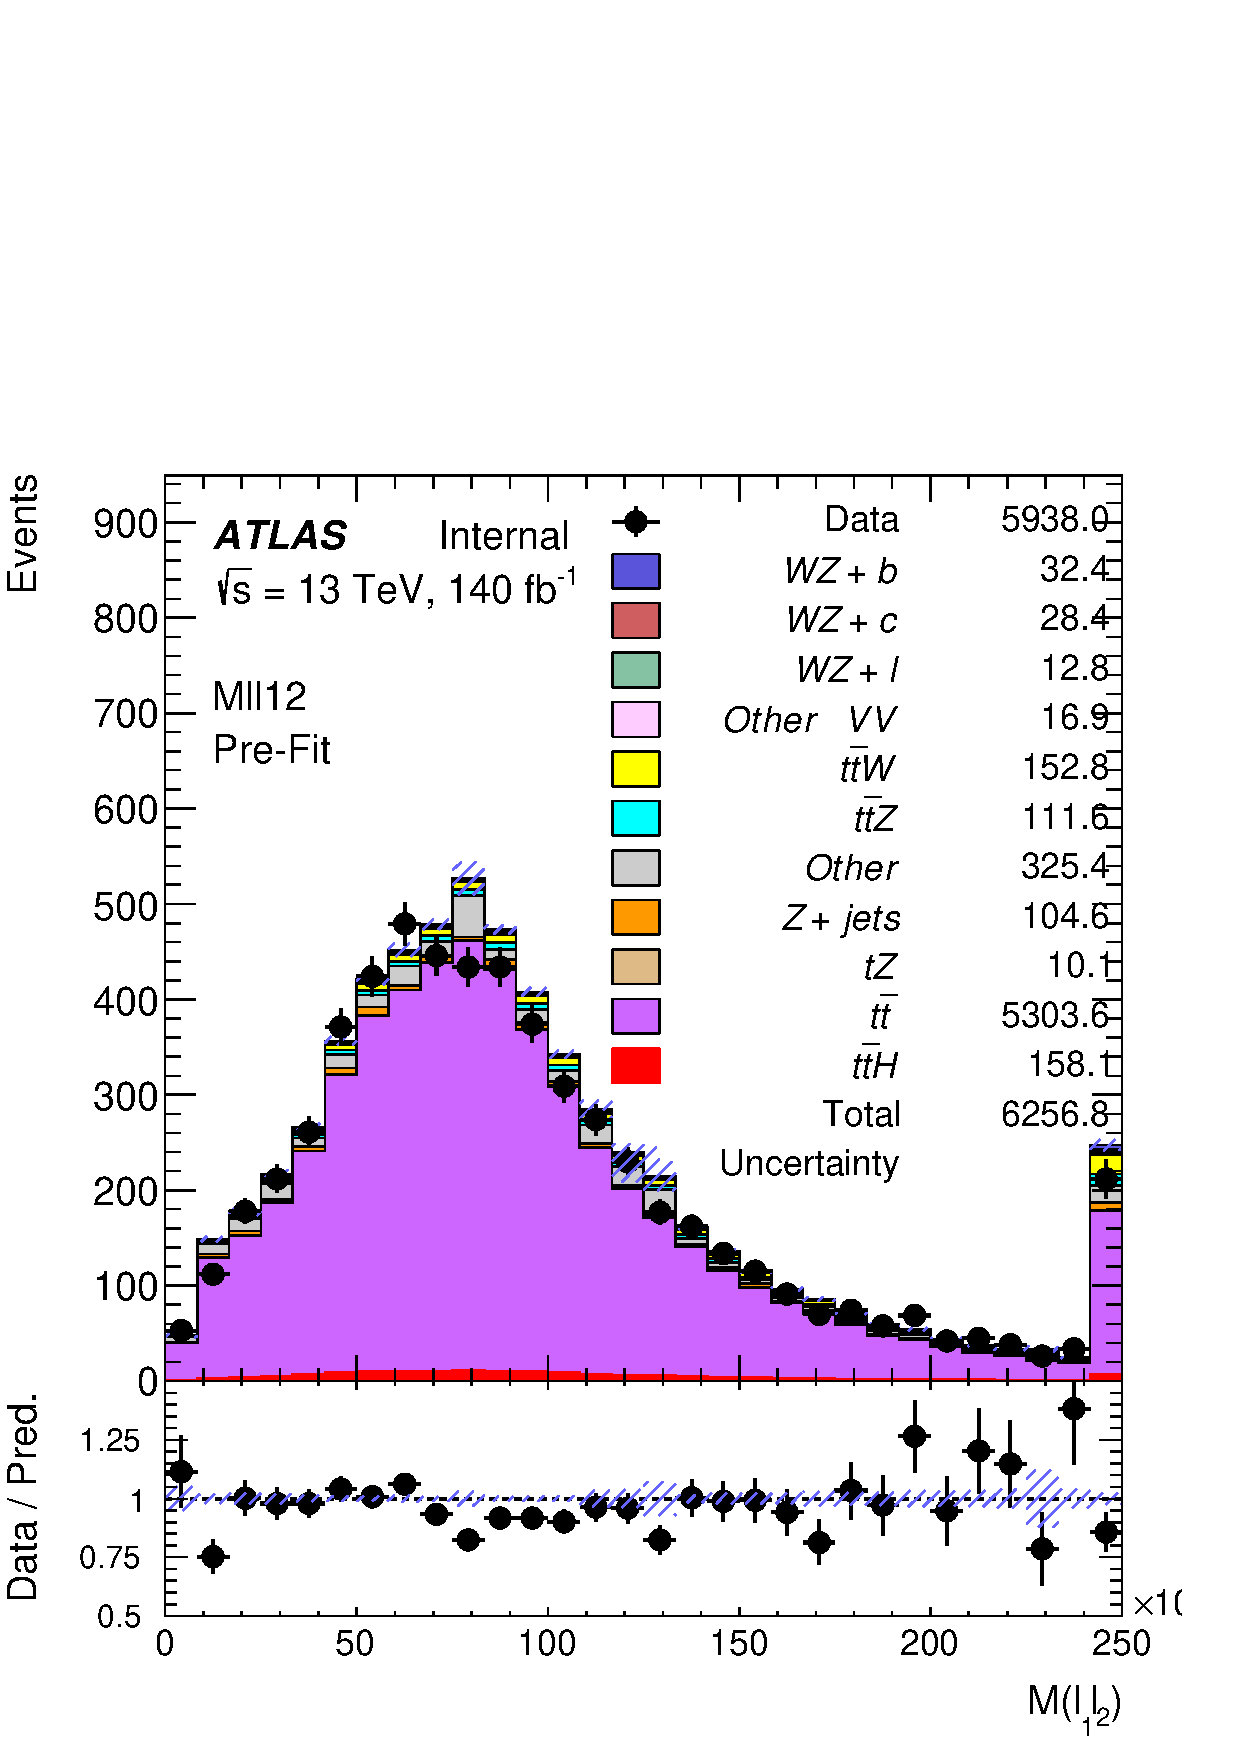
\includegraphics[width=.29\linewidth]{regions/plots_inclusive/Plots/Mll12.png}}%
    \caption{Comparisons between data and MC distributions in the preselection region for the $p_T$ of (a) the leading jet, (b) lepton 0, (c) lepton 1, (d) lepton 2, (e) the missing transverse energy, and (f) the invariant mass of leptons 0 and 1, (g) the invariant mass of leptons 0 and 2, and (h) the invariant mass of leptons 1 and 2.}
    \label{kin:inclusive}
\end{figure}

%---------------------------                                                                                         
\subsection{Fit Regions}
\label{subsec:regions}
%--------------------------- 

Once preselection has been applied, the remaining events are categorized into one of twelve orthogonal regions. The regions used in the fit are summarized in table \ref{tab:regions}.

\begin{table}[h]
\centering
\caption{A list of the regions used in the fit and the selection used for each.}
\begin{tabular}{l|l}
\hline\hline
Region & Selection            \\
\hline
\hline
%1j, <85\%       & $N_{jets}$ = 1, jet DL1r score < 85\% WP            \\
%1j, 85\%-77\%   & $N_{jets}$ = 1, 85\% < jet DL1r score < 77\% WP                    \\
%1j, 77\%-70\%   & $N_{jets}$ = 1, 77\% < jet DL1r score < 70\% WP                    \\
%1j, 70\%-60\%   & $N_{jets}$ = 1, 70\% < jet DL1r score < 60\% WP                    \\
%1j, >60\%       & $N_{jets}$ = 1, jet DL1r score > 85\% WP, tZ BDT score > 0.03 \\
%1j tZ CR        & $N_{jets}$ = 1, jet DL1r > 85\% WP, tZ BDT score < 0.03 \\
%2j, <85\%       & $N_{jets}$ = 2, jet DL1r score < 85\% WP                    \\
%2j, 85\%-77\%   & $N_{jets}$ = 2, 85\% WP < jet DL1r score < 77\% WP                 \\
%2j, 77\%-70\%   & $N_{jets}$ = 2, 77\% WP < jet DL1r score < 70\% WP                 \\
%2j, 70\%-60\%   & $N_{jets}$ = 2, 70\% < jet DL1r score < 60\% WP                     \\
%2j, >60\%       & $N_{jets}$ = 2, jet DL1r score > 85\% WP, tZ BDT score > 0.03 \\
%2j tZ CR        & $N_{jets}$ = 2, jet DL1r score > 85\% WP, tZ BDT score < 0.03 \\
1j, <85\%       & $N_{jets}$ = 1, nJets\_DL1r\_85 = 0            \\
1j, 85\%-77\%   & $N_{jets}$ = 1, nJets\_DL1r\_85 = 1, nJets\_DL1r\_77=0                     \\
1j, 77\%-70\%   & $N_{jets}$ = 1, nJets\_DL1r\_77 = 1, nJets\_DL1r\_70=0                     \\
1j, 70\%-60\%   & $N_{jets}$ = 1, nJets\_DL1r\_70 = 1, nJets\_DL1r\_60=0                      \\
1j, >60\%       & $N_{jets}$ = 1, nJets\_DL1r\_60 = 1, tZ BDT > 0.725 \\
1j tZ CR        & $N_{jets}$ = 1, nJets\_DL1r\_60 = 1, tZ BDT < 0.725 \\
2j, <85\%       & $N_{jets}$ = 2, nJets\_DL1r\_85 = 0                    \\
2j, 85\%-77\%   & $N_{jets}$ = 2, nJets\_DL1r\_85 >= 1, nJets\_DL1r\_77=0                     \\
2j, 77\%-70\%   & $N_{jets}$ = 2, nJets\_DL1r\_77 >= 1, nJets\_DL1r\_70=0                     \\
2j, 70\%-60\%   & $N_{jets}$ = 2, nJets\_DL1r\_70 >= 1, nJets\_DL1r\_60=0                      \\
2j, >60\%       & $N_{jets}$ = 2, nJets\_DL1r\_60 >= 1, tZ BDT > 0.725 \\
2j tZ CR        & $N_{jets}$ = 2, nJets\_DL1r\_60 >= 1, tZ BDT < 0.725 \\
\hline\hline
\end{tabular}
\label{tab:regions}
\end{table}

The working points discussed in section \ref{subsec:bjets} are used to separate events into fit regions based on the highest working point reached by a jet in each event. Because the background composition differs significantly based on the number of b-jets, events are further subdivided into 1 jet and 2 jet regions in order to minimize the impact of background uncertainties.

An additional tZ control region is created based on the BDT described in section \ref{sec:tZ_bdt}. The region with 1-jet passing the 60\% working point is split in two - a signal enriched region of events with a BDT score greater than 0.03, and a tZ control region including events with less than 0.03. This cutoff is arrived at by performing an Asimov fit with a variety of cutoffs, and selecting the value that produces the highest significance for the measurement of $WZ$ + b.

The modeling in each region is validated by comparing data and MC predictions for various kinematic distributions. These plot are shown in figures \ref{kin:WP_1j_not85}-\ref{kin:tZ_CR_2j}.

\begin{figure}[H]
    \centering
    \textbf{WZ Fit Region - 1j $<$ 85\% WP}\\
    \subfigure[]{\includegraphics[width=.29\linewidth]{regions/plots_not_85/Plots/lead_jetPt.png}}%
    \subfigure[]{\includegraphics[width=.29\linewidth]{regions/plots_not_85/Plots/lep_Pt_0.png}}%
    \subfigure[]{\includegraphics[width=.29\linewidth]{regions/plots_not_85/Plots/lep_Pt_1.png}}\\
    \subfigure[]{\includegraphics[width=.29\linewidth]{regions/plots_not_85/Plots/lep_Pt_2.png}}%
    \subfigure[]{\includegraphics[width=.29\linewidth]{regions/plots_not_85/Plots/MET.png}}%
    \subfigure[]{\includegraphics[width=.29\linewidth]{regions/plots_not_85/Plots/Mll01.png}}\\
    \caption{Comparisons between the data and MC distributions in the preselection region for the $p_T$ of (a) the leading jet, (b) lepton 0, (c) lepton 1, (d) lepton 2, (e) the missing transverse energy, and (f) the invariant mass of lepton 0 and 1.}
    \label{kin:WP_1j_not85}
\end{figure}

\begin{figure}[H]
    \centering
    \textbf{WZ Fit Region - 1j 77-85\% WP}\\
    \subfigure[]{\includegraphics[width=.29\linewidth]{regions/plots_1j_77_85/Plots/lead_jetPt.png}}%
    \subfigure[]{\includegraphics[width=.29\linewidth]{regions/plots_1j_77_85/Plots/lep_Pt_0.png}}%
    \subfigure[]{\includegraphics[width=.29\linewidth]{regions/plots_1j_77_85/Plots/lep_Pt_1.png}}\\
    \subfigure[]{\includegraphics[width=.29\linewidth]{regions/plots_1j_77_85/Plots/lep_Pt_2.png}}%
    \subfigure[]{\includegraphics[width=.29\linewidth]{regions/plots_1j_77_85/Plots/MET.png}}%
    \subfigure[]{\includegraphics[width=.29\linewidth]{regions/plots_1j_77_85/Plots/Mll01.png}}\\
    \caption{Comparisons between the data and MC distributions in the preselection region for the $p_T$ of (a) the leading jet, (b) lepton 0, (c) lepton 1, (d) lepton 2, (e) the missing transverse energy, and (f) the invariant mass of lepton 0 and 1.}
    \label{kin:WP_1j_77_85}
\end{figure}

\begin{figure}[H]
    \centering
    \textbf{WZ Fit Region - 1j 70-77\% WP}\\
    \subfigure[]{\includegraphics[width=.29\linewidth]{regions/plots_1j_70_77/Plots/lead_jetPt.png}}%
    \subfigure[]{\includegraphics[width=.29\linewidth]{regions/plots_1j_70_77/Plots/lep_Pt_0.png}}%
    \subfigure[]{\includegraphics[width=.29\linewidth]{regions/plots_1j_70_77/Plots/lep_Pt_1.png}}\\
    \subfigure[]{\includegraphics[width=.29\linewidth]{regions/plots_1j_70_77/Plots/lep_Pt_2.png}}%
    \subfigure[]{\includegraphics[width=.29\linewidth]{regions/plots_1j_70_77/Plots/MET.png}}%
    \subfigure[]{\includegraphics[width=.29\linewidth]{regions/plots_1j_70_77/Plots/Mll01.png}}\\
    \caption{Comparisons between the data and MC distributions in the preselection region for the $p_T$ of (a) the leading jet, (b) lepton 0, (c) lepton 1, (d) lepton 2, (e) the missing transverse energy, and (f) the invariant mass of lepton 0 and 1.}
    \label{kin:WP_1j_70_77}   
\end{figure}

\begin{figure}[H]
    \centering
    \textbf{WZ Fit Region - 1j 60-70\% WP}\\
    \subfigure[]{\includegraphics[width=.29\linewidth]{regions/plots_1j_60_70/Plots/lead_jetPt.png}}%
    \subfigure[]{\includegraphics[width=.29\linewidth]{regions/plots_1j_60_70/Plots/lep_Pt_0.png}}%
    \subfigure[]{\includegraphics[width=.29\linewidth]{regions/plots_1j_60_70/Plots/lep_Pt_1.png}}\\
    \subfigure[]{\includegraphics[width=.29\linewidth]{regions/plots_1j_60_70/Plots/lep_Pt_2.png}}%
    \subfigure[]{\includegraphics[width=.29\linewidth]{regions/plots_1j_60_70/Plots/MET.png}}%
    \subfigure[]{\includegraphics[width=.29\linewidth]{regions/plots_1j_60_70/Plots/Mll01.png}}\\
    \caption{Comparisons between the data and MC distributions in the preselection region for the $p_T$ of (a) the leading jet, (b) lepton 0, (c) lepton 1, (d) lepton 2, (e) the missing transverse energy, and (f) the invariant mass of lepton 0 and 1.}
    \label{kin:WP_1j_60_70}
\end{figure}

\begin{figure}[H]
    \centering
    \textbf{WZ Fit Region - 1j 60\% WP}\\
    \subfigure[]{\includegraphics[width=.29\linewidth]{regions/plots_1j_60/Plots/lead_jetPt.png}}%
    \subfigure[]{\includegraphics[width=.29\linewidth]{regions/plots_1j_60/Plots/lep_Pt_0.png}}%
    \subfigure[]{\includegraphics[width=.29\linewidth]{regions/plots_1j_60/Plots/lep_Pt_1.png}}\\
    \subfigure[]{\includegraphics[width=.29\linewidth]{regions/plots_1j_60/Plots/lep_Pt_2.png}}%
    \subfigure[]{\includegraphics[width=.29\linewidth]{regions/plots_1j_60/Plots/MET.png}}%
    \subfigure[]{\includegraphics[width=.29\linewidth]{regions/plots_1j_60/Plots/Mll01.png}}\\
    \caption{Comparisons between the data and MC distributions in the preselection region for the $p_T$ of (a) the leading jet, (b) lepton 0, (c) lepton 1, (d) lepton 2, (e) the missing transverse energy, and (f) the invariant mass of lepton 0 and 1.}
    \label{kin:WP_1j_60}    
\end{figure}

\begin{figure}[H]
    \centering
    \textbf{WZ Fit Region - tZ-CR}\\
    \subfigure[]{\includegraphics[width=.29\linewidth]{regions/plots_tZ_CR/Plots/lead_jetPt.png}}%
    \subfigure[]{\includegraphics[width=.29\linewidth]{regions/plots_tZ_CR/Plots/lep_Pt_0.png}}%
    \subfigure[]{\includegraphics[width=.29\linewidth]{regions/plots_tZ_CR/Plots/lep_Pt_1.png}}\\
    \subfigure[]{\includegraphics[width=.29\linewidth]{regions/plots_tZ_CR/Plots/lep_Pt_2.png}}%
    \subfigure[]{\includegraphics[width=.29\linewidth]{regions/plots_tZ_CR/Plots/MET.png}}%
    \subfigure[]{\includegraphics[width=.29\linewidth]{regions/plots_tZ_CR/Plots/Mll01.png}}\\
    \caption{Comparisons between the data and MC distributions in the preselection region for the $p_T$ of (a) the leading jet, (b) lepton 0, (c) lepton 1, (d) lepton 2, (e) the missing transverse energy, and (f) the invariant mass of lepton 0 and 1.}
    \label{kin:tZ_CR_1j}
\end{figure}

\begin{figure}[H]
    \centering
    \textbf{WZ Fit Region - 2j $<$ 85\% WP}\\
    \subfigure[]{\includegraphics[width=.29\linewidth]{regions/plots_not_85_2j/Plots/lead_jetPt.png}}%
    \subfigure[]{\includegraphics[width=.29\linewidth]{regions/plots_not_85_2j/Plots/lep_Pt_0.png}}%
    \subfigure[]{\includegraphics[width=.29\linewidth]{regions/plots_not_85_2j/Plots/lep_Pt_1.png}}\\
    \subfigure[]{\includegraphics[width=.29\linewidth]{regions/plots_not_85_2j/Plots/lep_Pt_2.png}}%
    \subfigure[]{\includegraphics[width=.29\linewidth]{regions/plots_not_85_2j/Plots/MET.png}}%
    \subfigure[]{\includegraphics[width=.29\linewidth]{regions/plots_not_85_2j/Plots/Mll01.png}}\\
    \caption{Comparisons between the data and MC distributions in the preselection region for the $p_T$ of (a) the leading jet, (b) lepton 0, (c) lepton 1, (d) lepton 2, (e) the missing transverse energy, and (f) the invariant mass of lepton 0 and 1.}
    \label{kin:WP_2j_not85}
\end{figure}

\begin{figure}[H]
    \centering
    \textbf{WZ Fit Region - 2j 77-85\% WP}\\
    \subfigure[]{\includegraphics[width=.29\linewidth]{regions/plots_2j_77_85/Plots/lead_jetPt.png}}%
    \subfigure[]{\includegraphics[width=.29\linewidth]{regions/plots_2j_77_85/Plots/lep_Pt_0.png}}%
    \subfigure[]{\includegraphics[width=.29\linewidth]{regions/plots_2j_77_85/Plots/lep_Pt_1.png}}\\
    \subfigure[]{\includegraphics[width=.29\linewidth]{regions/plots_2j_77_85/Plots/lep_Pt_2.png}}%
    \subfigure[]{\includegraphics[width=.29\linewidth]{regions/plots_2j_77_85/Plots/MET.png}}%
    \subfigure[]{\includegraphics[width=.29\linewidth]{regions/plots_2j_77_85/Plots/Mll01.png}}\\
    \caption{Comparisons between the data and MC distributions in the preselection region for the $p_T$ of (a) the leading jet, (b) lepton 0, (c) lepton 1, (d) lepton 2, (e) the missing transverse energy, and (f) the invariant mass of lepton 0 and 1.}
    \label{kin:WP_2j_77_85}
\end{figure}

\begin{figure}[H]
    \centering
    \textbf{WZ Fit Region - 2j 70-77\% WP}\\
    \subfigure[]{\includegraphics[width=.29\linewidth]{regions/plots_2j_70_77/Plots/lead_jetPt.png}}%
    \subfigure[]{\includegraphics[width=.29\linewidth]{regions/plots_2j_70_77/Plots/lep_Pt_0.png}}%
    \subfigure[]{\includegraphics[width=.29\linewidth]{regions/plots_2j_70_77/Plots/lep_Pt_1.png}}\\
    \subfigure[]{\includegraphics[width=.29\linewidth]{regions/plots_2j_70_77/Plots/lep_Pt_2.png}}%
    \subfigure[]{\includegraphics[width=.29\linewidth]{regions/plots_2j_70_77/Plots/MET.png}}%
    \subfigure[]{\includegraphics[width=.29\linewidth]{regions/plots_2j_70_77/Plots/Mll01.png}}\\
    \caption{Comparisons between the data and MC distributions in the preselection region for the $p_T$ of (a) the leading jet, (b) lepton 0, (c) lepton 1, (d) lepton 2, (e) the missing transverse energy, and (f) the invariant mass of lepton 0 and 1.}
    \label{kin:WP_2j_70_77}
\end{figure}

\begin{figure}[H]
    \centering
    \textbf{WZ Fit Region - 2j 60-70\% WP}\\
    \subfigure[]{\includegraphics[width=.29\linewidth]{regions/plots_2j_60_70/Plots/lead_jetPt.png}}%
    \subfigure[]{\includegraphics[width=.29\linewidth]{regions/plots_2j_60_70/Plots/lep_Pt_0.png}}%
    \subfigure[]{\includegraphics[width=.29\linewidth]{regions/plots_2j_60_70/Plots/lep_Pt_1.png}}\\
    \subfigure[]{\includegraphics[width=.29\linewidth]{regions/plots_2j_60_70/Plots/lep_Pt_2.png}}%
    \subfigure[]{\includegraphics[width=.29\linewidth]{regions/plots_2j_60_70/Plots/MET.png}}%
    \subfigure[]{\includegraphics[width=.29\linewidth]{regions/plots_2j_60_70/Plots/Mll01.png}}\\
    \caption{Comparisons between the data and MC distributions in the preselection region for the $p_T$ of (a) the leading jet, (b) lepton 0, (c) lepton 1, (d) lepton 2, (e) the missing transverse energy, and (f) the invariant mass of lepton 0 and 1.}
    \label{kin:WP_2j_60_70}
\end{figure}

\begin{figure}[H]
    \centering
    \textbf{WZ Fit Region - 2j 60\% WP}\\
    \subfigure[]{\includegraphics[width=.29\linewidth]{regions/plots_2j_60/Plots/lead_jetPt.png}}%
    \subfigure[]{\includegraphics[width=.29\linewidth]{regions/plots_2j_60/Plots/lep_Pt_0.png}}%
    \subfigure[]{\includegraphics[width=.29\linewidth]{regions/plots_2j_60/Plots/lep_Pt_1.png}}\\
    \subfigure[]{\includegraphics[width=.29\linewidth]{regions/plots_2j_60/Plots/lep_Pt_2.png}}%
    \subfigure[]{\includegraphics[width=.29\linewidth]{regions/plots_2j_60/Plots/MET.png}}%
    \subfigure[]{\includegraphics[width=.29\linewidth]{regions/plots_2j_60/Plots/Mll01.png}}\\
    \caption{Comparisons between the data and MC distributions in the preselection region for the $p_T$ of (a) the leading jet, (b) lepton 0, (c) lepton 1, (d) lepton 2, (e) the missing transverse energy, and (f) the invariant mass of lepton 0 and 1.}
    \label{kin:WP_2j_60}
\end{figure}

\begin{figure}[H]
    \textbf{WZ Fit Region - tZ-CR-2j}\\
    \subfigure[]{\includegraphics[width=.29\linewidth]{regions/plots_tZ_CR_2j/Plots/lead_jetPt.png}}%
    \subfigure[]{\includegraphics[width=.29\linewidth]{regions/plots_tZ_CR_2j/Plots/lep_Pt_0.png}}%
    \subfigure[]{\includegraphics[width=.29\linewidth]{regions/plots_tZ_CR_2j/Plots/lep_Pt_1.png}}\\
    \subfigure[]{\includegraphics[width=.29\linewidth]{regions/plots_tZ_CR_2j/Plots/lep_Pt_2.png}}%
    \subfigure[]{\includegraphics[width=.29\linewidth]{regions/plots_tZ_CR_2j/Plots/MET.png}}%
    \subfigure[]{\includegraphics[width=.29\linewidth]{regions/plots_tZ_CR_2j/Plots/Mll01.png}}\\
    \caption{Comparisons between the data and MC distributions in the preselection region for the $p_T$ of (a) the leading jet, (b) lepton 0, (c) lepton 1, (d) lepton 2, (e) the missing transverse energy, and (f) the invariant mass of lepton 0 and 1.}
    \label{kin:tZ_CR_2j}
\end{figure}

%---------------------------
\subsection{Non-Prompt Lepton Estimation}
\label{sec:fakes}
%---------------------------

Two processes act as sources of non-prompt leptons appear in the analysis: $t\bar{t}$ and $Z$+jet production both produce two prompt leptons, and each contribute to the 3l region when an additional non-prompt lepton appears in the event. The contribution of these processes is estimated with Monte Carlo simulations, which are validated using enriched validation regions.

\subsubsection{$t\bar{t}$ Validation}

$t\bar{t}$ events can produce two prompt leptons from the decay of each of the tops. These top decays produce two b-quarks, the decay of which can produce additional non-prompt leptons, which occasionally pass the event preselection. In order to validate that the Monte Carlo accurately simulates this process accurately, the MC prediction in a non-prompt $t\bar{t}$ enriched validation region is compared to data.

The $t\bar{t}$ validation region is similar to the preselection region - three leptons meeting the criteria described in section \ref{sec:evt_selection} are required, and the requirements on $E_T^{miss}$ remain the same. However, the selection requiring a lepton pair form a Z-candidate are reversed. Events where the invariant mass of any two opposite sign, same flavor leptons falls within 10 GeV of 91.2 GeV are rejected. This ensures the $t\bar{t}$ validation region is orthogonal to the preselection region. 

Further, because the jet multiplicity of $t\bar{t}$ events tends to be higher than WZ, the number of jets in each event is required to be greater than 1. As b-jets are almost invariably produced from top decays, at least one b-tagged jet passing the 70\% DL1r WP in each event is required. Various kinematic plots of this region are shown in figure \ref{fig:ttbar_noScale}.

\begin{figure}[H]
    \centering
    \subfigure[]{\includegraphics[width=0.29\textwidth]{ttbar/noScale/lead_jetPt.png}}%                             
    \subfigure[]{\includegraphics[width=0.29\textwidth]{ttbar/noScale/MET.png}}%
    \subfigure[]{\includegraphics[width=0.29\textwidth]{ttbar/noScale/lep_Pt_0.png}}\\
    \subfigure[]{\includegraphics[width=0.29\textwidth]{ttbar/noScale/lep_Pt_1.png}}%
    \subfigure[]{\includegraphics[width=0.29\textwidth]{ttbar/noScale/lep_Pt_2.png}}%                                                 
    \subfigure[]{\includegraphics[width=0.29\textwidth]{ttbar/noScale/Mll01.png}}\\
    \subfigure[]{\includegraphics[width=0.29\textwidth]{ttbar/noScale/Mll02.png}}%
    \subfigure[]{\includegraphics[width=0.29\textwidth]{ttbar/noScale/nJets_OR.png}}%                                       
    \subfigure[]{\includegraphics[width=0.29\textwidth]{ttbar/noScale/nJets_OR_DL1r_70.png}}\\
    \caption{Comparisons between the data and MC distributions in the $t\bar{t}$ validation region for (a) the $p_T$ of the leading jet, (b) the missing transverse energy, (c) the $p_T$ of lepton 0, (d) $p_T$ of lepton 1, (e) $p_T$ of lepton 2, (f) the invariant mass of leptons 0 and 1, (g) the invariant mass of leptons 0 and 2, (h) the number of jets, (i) the number of b-tagged jets.}
    \label{fig:ttbar_noScale}
\end{figure}

The shape of each distribution agrees quite well between data and MC, with a constant offset between the two. This is accounted for by applying a constant correction factor of 0.883 to the $t\bar{t}$ MC prediction. Plots showing the kinematics of the $t\bar{t}$ VR after this correction factor has been applied are shown in figure \ref{fig:ttbar_withScale}.

\begin{figure}[H]
    \centering
    \subfigure[]{\includegraphics[width=0.29\textwidth]{ttbar/withScale/lead_jetPt.png}}%                                    
    \subfigure[]{\includegraphics[width=0.29\textwidth]{ttbar/withScale/MET.png}}%                                           
    \subfigure[]{\includegraphics[width=0.29\textwidth]{ttbar/withScale/lep_Pt_0.png}}\\                                     
    \subfigure[]{\includegraphics[width=0.29\textwidth]{ttbar/withScale/lep_Pt_1.png}}%                                      
    \subfigure[]{\includegraphics[width=0.29\textwidth]{ttbar/withScale/lep_Pt_2.png}}%                            
    \subfigure[]{\includegraphics[width=0.29\textwidth]{ttbar/withScale/Mll01.png}}\\                                        
    \subfigure[]{\includegraphics[width=0.29\textwidth]{ttbar/withScale/Mll02.png}}%                                         
    \subfigure[]{\includegraphics[width=0.29\textwidth]{ttbar/withScale/nJets_OR.png}}%                                      
    \subfigure[]{\includegraphics[width=0.29\textwidth]{ttbar/withScale/nJets_OR_DL1r_70.png}}\\                             
    \caption{Comparisons between the data and MC distributions in the $t\bar{t}$ validation region after the correction factor has been applied for (a) the $p_T$ of the leading jet, (b) the missing transverse energy, (c) the $p_T$ of lepton 0, (d) $p_T$ of lepton 1, (e) $p_T$ of lepton 2, (f) the invariant mass of leptons 0 and 1, (g) the invariant mass of leptons 0 and 2, (h) the number of jets, (i) the number of b-tagged jets.}                                                                   
     \label{fig:ttbar_withScale}
\end{figure}

The modeling is further validated by looking at the yield in the $t\bar{t}$ VR for each DL1r WP, giving a clearer correspondence to the signal regions used in the fit. Each region shown in figure \ref{fig:ttbar_summary} requires one or more jets pass the listed WP, with no jets passing the next highest WP.

\begin{figure}[H]
   \centering
   \includegraphics[width=0.9\textwidth]{ttbar/Summary.png}   
   \caption{Data and MC comparisons for each DL1r WP for both 1-jet and 2-jet regions, after the $t\bar{t}$ VR selection and correction factor have been applied}
   \label{fig:ttbar_summary}
\end{figure}

As data and MC are found to agree within 10\% for each of these working points, a 10\% systematic uncertainty on the $t\bar{t}$ prediction is included for the analysis.

\subsubsection{$Z$+jets Validation}

Similar to $t\bar{t}$, a non-prompt $Z$+jets validation region is produced in order to validate the MC predictions. The lepton requirements remain the same as the preselection region. Because no neutrinos are present for this process, the $E_T^{miss}$ cut is reversed, requiring $E_T^{miss}$ < 30 GeV. This also ensures this validation region is orthogonal to the preselection region. Further, the number of jets in each event is required to be greater than or equal to one. Various kinematic plots of this region are shown below. The general agreement between data and MC in each of these suggests that the non-prompt contribution of $Z$+jets is well modeled by Monte Carlo.

\begin{figure}[H]
    \subfigure[]{\includegraphics[width=0.29\textwidth]{zjets/noScale/lead_jetPt.png}}%                          
    \subfigure[]{\includegraphics[width=0.29\textwidth]{zjets/noScale/DRll01.png}}%
    \subfigure[]{\includegraphics[width=0.29\textwidth]{zjets/noScale/lep_Pt_0.png}}\\
    \subfigure[]{\includegraphics[width=0.29\textwidth]{zjets/noScale/lep_Pt_1.png}}%
    \subfigure[]{\includegraphics[width=0.29\textwidth]{zjets/noScale/lep_Pt_2.png}}%                                      
    \subfigure[]{\includegraphics[width=0.29\textwidth]{zjets/noScale/Mll01.png}}\\
    \subfigure[]{\includegraphics[width=0.29\textwidth]{zjets/noScale/Mll02.png}}%
    \subfigure[]{\includegraphics[width=0.29\textwidth]{zjets/noScale/nJets_OR.png}}%                            
    \subfigure[]{\includegraphics[width=0.29\textwidth]{zjets/noScale/DRll02.png}}\\
    \caption{Comparisons between the data and MC distributions in the $Z$+jets validation region for (a) the $p_T$ of the leading jet, (b) $\Delta R$ between leptons 0 and 1, (c) the $p_T$ of lepton 0, (d) $p_T$ of lepton 1, (e) $p_T$ of lepton 2, (f) the invariant mass of leptons 0 and 1, (g) the invariant mass of leptons 0 and 2, (h) the number of jets, (i) $\Delta R$ between leptons 0 and 2. Includes only statistical uncertainties}%(i) the number of b-tagged jets.}
    \label{fig:zjets_noScale}
\end{figure}

While there is general agreement between data and MC within statistical uncertainty, the shape of the $p_T$ spectrum of lepton 2 is found to differ. To account for this discrepency, a variable correction factor is applied to Z+jets. $\chi^2$ minimization of the lepton 2 $p_T$ spectrum is performed to derive a correction factor of $1.53 - 6.6*10^{-6} (lep\_Pt\_2)$. Kinematic plots of the Z + jets validation region after this correction factor has been apllied are shown in figure \ref{fig:zjets_withScale}.

\begin{figure}[H]
    \subfigure[]{\includegraphics[width=0.29\textwidth]{zjets/withScale/lead_jetPt.png}}%              
    \subfigure[]{\includegraphics[width=0.29\textwidth]{zjets/withScale/DRll01.png}}%                            
    \subfigure[]{\includegraphics[width=0.29\textwidth]{zjets/withScale/lep_Pt_0.png}}\\
    \subfigure[]{\includegraphics[width=0.29\textwidth]{zjets/withScale/lep_Pt_1.png}}%                           
    \subfigure[]{\includegraphics[width=0.29\textwidth]{zjets/withScale/lep_Pt_2.png}}%                             
    \subfigure[]{\includegraphics[width=0.29\textwidth]{zjets/withScale/Mll01.png}}\\                                 
    \subfigure[]{\includegraphics[width=0.29\textwidth]{zjets/withScale/Mll02.png}}%                                   
    \subfigure[]{\includegraphics[width=0.29\textwidth]{zjets/withScale/nJets_OR.png}}%                               
    \subfigure[]{\includegraphics[width=0.29\textwidth]{zjets/withScale/DRll02.png}}\\
    \caption{Comparisons between the data and MC distributions in the $Z$+jets validation region after the correction factor has been applied for (a) the $p_T$ of the leading jet, (b) $\Delta R$ between leptons 0 and 1, (c) the $p_T$ of lepton 0, (d) $p_T$ of lepton 1, (e) $p_T$ of lepton 2, (f) the invariant mass of leptons 0 and 1, (g) the invariant mass of leptons 0 and 2, (h) the number of jets, (i) $\Delta R$ between leptons 0 and 2}%(i) the number of b-tagged jets.}                 
    \label{fig:zjets_noScale}
\end{figure}

The modeling is further validated by looking at the yield in the Z+jets VR for each DL1r WP, giving a clearer correspondence to the signal regions used in the fit. Each region shown in figure \ref{fig:ttbar_summary} requires one or more jets pass the listed WP, with no jets passing the next highest WP.                                                                    

                                                                                                                             
\begin{figure}[H]                                                                                                            
   \centering
   \includegraphics[width=0.9\textwidth]{zjets/Summary.png}
   \caption{Data and MC comparisons for each DL1r WP for both 1-jet and 2-jet regions, after the Z+jets VR selection and correction factor have been applied}                                                                                             
   \label{fig:ttbar_summary}
\end{figure}

For each of the working points considered, the data falls within 20\% of the MC prediction once this correction factor has been applied. Therefore, a 20\% systematic uncertainty is applied to Z + jets in the analysis.
